\documentclass[twocolumn, 12pt]{article}
\usepackage[utf8]{inputenc}
\usepackage{amsmath}
%\usepackage{marvosym}
\usepackage{textcomp}
\usepackage{geometry}
\usepackage{array}
\usepackage{wrapfig}
\usepackage{multirow}
\usepackage{graphicx}
\usepackage{float}
\usepackage{wrapfig}
\usepackage{caption}
\usepackage{amssymb}
\usepackage{ulem}
\usepackage[table]{xcolor}

\geometry{margin=.5in}

\begin{document}
\small

\section*{Heat Transfer Final}

%%%%%%%%%%%%%%%%%%%%%%%%
\subsection*{Heat Exchangers}

\begin{equation*}
    R_{tot} \triangleq \frac{1}{UA} \Rightarrow \frac{1}{UA} + \frac{1}{h_cA_c} + \frac{R_{f,c}''}{A_c} + R_{w,cond} + \frac{R_{f,h}''}{A_h} + \frac{1}{h_hA_h}
\end{equation*}
\begin{center}
    (see table 11.1)
\end{center}
\begin{equation*}
    \Dot{m}_h C_{p,h} (T_{h,i} -T_{h,o}) = q = \Dot{m}_c C_{p,c} (T_{c,o} -T_{c,i})
\end{equation*}

%%%%%%%%%%%%%%%%%%%%%%%%
\subsubsection*{LMTD}
\begin{equation*}
    q = UA \Delta T_{lm} = UA \frac{\Delta T_2 - \Delta T_1}{ln\left(\Delta T_2 / \Delta T_1 \right)}  
\end{equation*}
\underline{Concentric Parallel Flow}
\begin{equation*}
    \Delta T_1 \triangleq T_{h,i} - T_{c,i} \hspace{30pt} \Delta T_2 \triangleq T_{h,o} - T_{c,o}
\end{equation*}
\underline{Concentric Counter Flow}
\begin{equation*}
    \Delta T_1 \triangleq T_{h,o} - T_{c,i} \hspace{30pt} \Delta T_2 \triangleq T_{h,i} - T_{c,o}
\end{equation*}
\noindent
For the same inlet and outlet temps \(\Delta T_{lm\perp} > \Delta T_{lm \parallel}\)


%%%%%%%%%%%%%%%%%%%%%%%%
\subsubsection*{NTU}
\begin{equation*}
    \varepsilon \triangleq \frac{q}{q_{max}} \hspace{30pt} q = \varepsilon q_{max} = \varepsilon C_{min} (T_{h,i} - T_{c,i})
\end{equation*}
\begin{equation*}
    \varepsilon  = f(NTU, Cr) \hspace{30pt} Cr \triangleq \frac{C_{min}}{C_{max}} \hspace{30pt} NTU \triangleq \frac{UA}{C_{min}}
\end{equation*}
\begin{center}
    For \(Cr=0\) (all HE)    \(\Rightarrow\hspace{10pt}\varepsilon = 1 -exp(-NTU)\)
\end{center}
%%%%%%%%%%%%%%%%%%%%%%%%
\subsection*{Radiation}
\begin{itemize}
    \item \underline{Reflectivity} \(\rho\): Fraction of G that is reflected by the surface
    \item \underline{Absorptivity} \(\alpha\): Fraction of G that is absorbed by the surface
    \item \underline{Transmissivity} \(\tau\): Fraction of G that is transmitted by the surface (\(\tau =0\) in this course)
\end{itemize}
\begin{figure}[h]
    \centering
    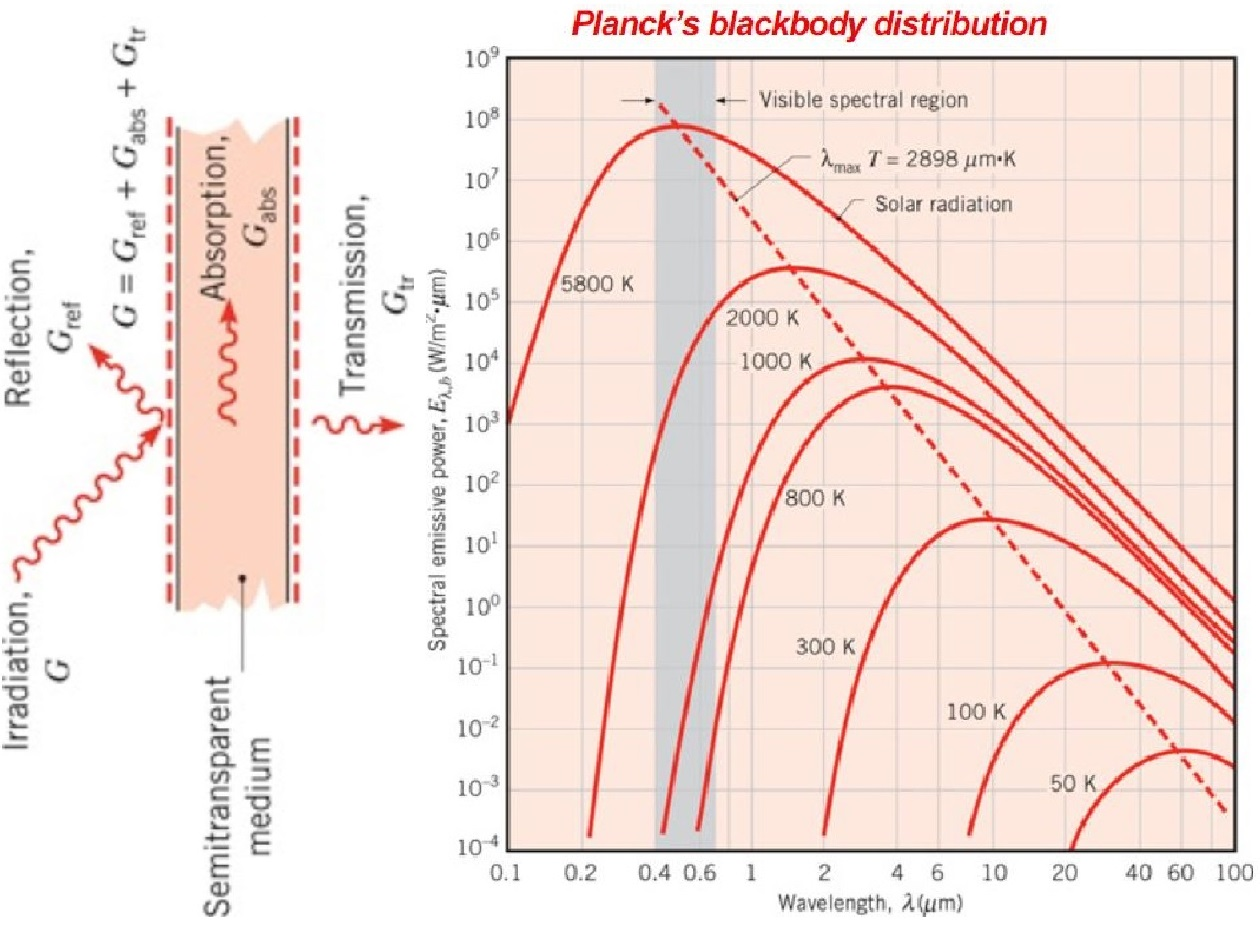
\includegraphics[scale=0.35]{RadiationGraphicPlusPlacksDistribution.jpg}
    \label{fig:RadiationGraphicPlusPlacksDistribution}
\end{figure}
\begin{equation*}
    J = E + G_{ref} \hspace{30pt} q_{rad}''= \varepsilon\sigma T_s^4 - \alpha G
\end{equation*}
\begin{equation*}
    d\omega = sin\theta d\theta d\phi \hspace{30pt} \omega_{hemisphere} = 2\pi \hspace{7.5pt} [Sr]
\end{equation*}
%%%
\underline{Radiative Intensity}
\begin{equation*}
    I_{\lambda,e} (\lambda,\theta,\phi) = \frac{dq}{ dA_1cos\theta d\omega d\lambda}  \hspace{7.5pt} \left[ \frac{W}{m^2 \cdot Sr\cdot \mu m} \right]
\end{equation*}
\underline{Spectral Heat Rate and Flux}
\begin{equation*}
    dq_\lambda =\frac{dq}{d\lambda} = I_{\lambda,e} (\lambda,\theta,\phi) cos \theta sin \theta d\theta d\phi \hspace{7.5pt} \left[ \frac{W}{\mu m} \right]
\end{equation*}
\begin{equation*}
    dq_\lambda'' =\frac{dq_\lambda}{dA_1} = I_{\lambda,e} (\lambda,\theta,\phi) cos \theta d\omega \hspace{7.5pt} \left[ \frac{W}{m^2 \cdot \mu m} \right]
\end{equation*}
%%%
\underline{Spectral and Total Emissive Power}
\begin{equation*}
    E_\lambda =q_\lambda'' = \int_{\phi=0}^{2\pi} \int_{\theta=0}^{\pi/2} I_{\lambda,e} (\lambda,\theta,\phi) cos \theta sin \theta d\theta d\phi \hspace{5pt} \left[ \frac{W}{m^2 \cdot \mu m} \right]
\end{equation*}
\begin{equation*}
    E = \int_{\lambda=0}^\infty E_\lambda d\lambda = \varepsilon \sigma T_s^4 \hspace{7.5pt} \left[ \frac{W}{m^2} \right]
\end{equation*}
\begin{equation*}
     E = \int_{\lambda=0}^\infty \int_{\phi=0}^{2\pi}  \int_{\theta=0}^{\pi/2} I_{\lambda,e} (\lambda,\theta,\phi) cos \theta sin \theta d\theta d\phi d\lambda 
\end{equation*}
\begin{center}
   If the emitter is diffuse \(\hspace{5pt} \Longrightarrow  \hspace{5pt} E_\lambda = \pi I_{\lambda,e}(\lambda)\) 
\end{center}
%%%
\underline{Spectral and Total Irradiation}
\begin{equation*}
    G_\lambda =  \int_{\phi=0}^{2\pi}  \int_{\theta=0}^{\pi/2} I_{\lambda,i} (\lambda,\theta,\phi) cos \theta sin \theta d\theta d\phi \hspace{7.5pt} \left[ \frac{W}{m^2 \cdot \mu m} \right]
\end{equation*}
\begin{equation*}
    G = \int_{\lambda=0}^\infty \int_{\phi=0}^{2\pi}  \int_{\theta=0}^{\pi/2} I_{\lambda,i} (\lambda,\theta,\phi) cos \theta sin \theta d\theta d\phi d\lambda \hspace{7.5pt} \left[ \frac{W}{m^2} \right]
\end{equation*}
\begin{center}
   If the surface is diffuse \(\hspace{2.5pt} \Rightarrow  \hspace{2.5pt} G_\lambda = \pi I_{\lambda,i}(\lambda)\) and \(G=\pi I_i\)
\end{center}
%%%
\underline{Spectral and Total Radiosity}
\begin{equation*}
    J_\lambda = \int_{\phi=0}^{2\pi}  \int_{\theta=0}^{\pi/2} I_{\lambda,e+r} (\lambda,\theta,\phi) cos \theta sin \theta d\theta d\phi \hspace{7.5pt} \left[ \frac{W}{m^2 \cdot \mu m} \right]
\end{equation*}
\begin{equation*}
    J = \int_{\lambda=0}^\infty \int_{\phi=0}^{2\pi}  \int_{\theta=0}^{\pi/2} I_{\lambda,e+r} (\lambda,\theta,\phi) cos \theta sin \theta d\theta d\phi d\lambda \hspace{7.5pt} \left[ \frac{W}{m^2} \right]
\end{equation*}
\begin{center}
   If the reflector and emitter are diffuse \(\hspace{2.5pt} \Rightarrow  \hspace{2.5pt} J_\lambda = \pi I_{\lambda,e+r}(\lambda)\) 
\end{center}


%%%%%%%%%%%%%%%%%%%%%%%%
\subsubsection*{Blackbody}
\begin{itemize}
    \item Absorbs \textbf{all} incident radiation
    \item No surface can emit more energy than a blackbody for a prescribed temperature and wavelength
    \item Blackbody emission \(=f(\lambda ,T)\) and \(\neq f(\theta,\phi )\)  
\end{itemize}
\begin{equation*}
    I_{\lambda,b} (\lambda, T) = \frac{2hc_o^2  }{ \lambda^5 [exp(hc_o/\lambda k_B T)^{-1}]}\hspace{7.5pt} \left[ \frac{W}{m^2 \cdot Sr \cdot \mu m} \right]
\end{equation*}
\underline{Where}:\\
\hspace{-20pt}
\begin{tabular}{|c c c l|}
    \hline
    \(h\) =& \(6.626 \times 10^{-34}\) &\([Js]\) &= Planck's Const.\\
    \(k_B\) =& \(1.581\times 10 ^ {-23}\)& \([J/K]\) &= Boltzman's Const.\\
    \(c_o\) =& \(2.998 \times 10^8 \)& \([m/s]\) &= Speed of light\\
    \(T\) =& problem subject & \([K]\) &= Temperature\\
    \hline
\end{tabular}
\begin{equation*}
     E_b = \int_{\lambda=0}^\infty E_{\lambda,b} d\lambda = \sigma T^4 \hspace{30pt}I_b = \frac{E_b}{\pi} = \frac{\sigma T^4}{\pi}
\end{equation*}
\begin{equation*}
    \text{Wien's Law} \hspace{30pt} \lambda_{max}T = 2898 \mu m K  
\end{equation*}
%%%
\underline{Band Emission}
\begin{equation*}
    F_{0->\lambda} = \frac{\int_0^\lambda E_{\lambda,b} d\lambda}{\int_0^\infty E_{\lambda,b} d\lambda} \hspace{20pt} \text{Tabulated, see table 12.2}
\end{equation*}


%%%%%%%%%%%%%%%%%%%%%%%%
\subsection*{Radiative Properties}
\underline{Spectral Directional Emissivity}
\begin{equation*}
    \varepsilon_{\lambda, \theta} (\lambda, \theta, \phi, T) = \frac{I_{\lambda, e} (\lambda, \theta, \phi, T)}{I_{\lambda,b} (\lambda, T)}
\end{equation*}
\underline{Spectral Emissivity}
\begin{equation*}
    \varepsilon_\lambda =\frac{E_\lambda}{E_{\lambda,b}} = \frac{ \int_{\phi=0}^{2\pi} \int_{\theta=0}^{\pi/2} I_{\lambda,e} (\lambda,\theta,\phi) cos \theta sin \theta d\theta d\phi}{\int_{\phi=0}^{2\pi} \int_{\theta=0}^{\pi/2} I_{\lambda,b} (\lambda,\theta,\phi) cos \theta sin \theta d\theta d\phi}
\end{equation*}
\underline{Total Emissivity}
\begin{equation*}
    \varepsilon = \frac{\int_0^\infty \varepsilon_{\lambda,b} E_{\lambda,b} d\lambda}{\int_0^\infty E_{\lambda,b} d\lambda} = \frac{\int_0^\infty \varepsilon_{\lambda,b} E_{\lambda,b} d\lambda}{E_b}
\end{equation*}
%%%
\underline{Spectral Directional Absorptivity}
\begin{equation*}
    \alpha_{\lambda,\theta} (\lambda, \theta, \phi) = \frac{I_{\lambda,i,abs} (\lambda, \theta, \phi)}{I_{\lambda,i} (\lambda, \theta, \phi)}
\end{equation*}
%%%
\underline{Spectral Absorptivity}
\begin{equation*}
    \alpha_{\lambda}(\lambda) = \frac{G_{\lambda,abs}(\lambda)}{G_{\lambda}(\lambda)} = \frac{\int_{\phi=0}^{2\pi}  \int_{\theta=0}^{\pi/2} \alpha_{\lambda,\theta} I_{\lambda,i,abs}  cos \theta sin \theta d\theta d\phi }{\int_{\phi=0}^{2\pi}  \int_{\theta=0}^{\pi/2}  I_{\lambda,i,abs}  cos \theta sin \theta d\theta d\phi}
\end{equation*}
%%%
\underline{Diffuse Irradiation}
\begin{equation*}
    \alpha(\lambda,T) = \frac{1}{\pi} \int_{\phi=0}^{2\pi}  \int_{\theta=0}^{\pi/2} \alpha(\lambda,\theta) cos \theta sin \theta d\theta d\phi
\end{equation*}
\begin{center}
    If the surface is diffuse \(\Longrightarrow \alpha_\lambda = \alpha_{\lambda,\theta}\)
\end{center}
%%%
\underline{Total Absorptivity}
\begin{equation*}
    \alpha = \frac{G_{abs} }{G} = \frac{\int_0^\infty \alpha_\lambda (\lambda) G_\lambda (\lambda) d\lambda}{\int_0^\infty G_\lambda(\lambda) d\lambda}
\end{equation*}


%%%%%%%%%%%%%%%%%%%%%%%%
\subsubsection*{Kirchhoff's Law}
\underline{Always}\( \hspace{165pt}\Rightarrow\varepsilon_{\lambda,\theta} = \alpha_{\lambda,\theta}\)\\
\underline{if} (diffuse irradiation OR diffuse surface)
\(\Rightarrow\hspace{7pt}\varepsilon_\lambda = \alpha_\lambda\)\\
\underline{if} (G is blackbody OR surface is GREY)
\(\Rightarrow\hspace{13pt}\varepsilon = \alpha\)

%%%%%%%%%%%%%%%%%%%%%%%%
\vspace{-5pt}
\begin{figure}[h]
    \centering
    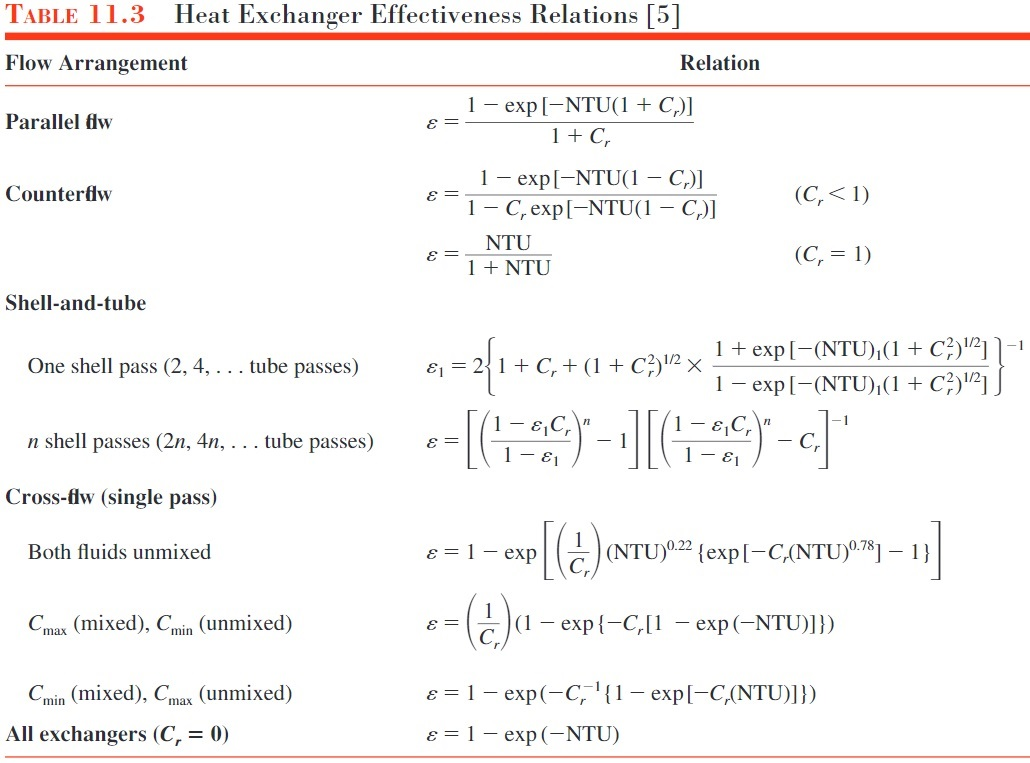
\includegraphics[scale=0.40]{Table11_3.jpg}
    \label{fig:Table113}
\end{figure}
\vspace{-20pt}
\begin{figure}[h]
    \centering
    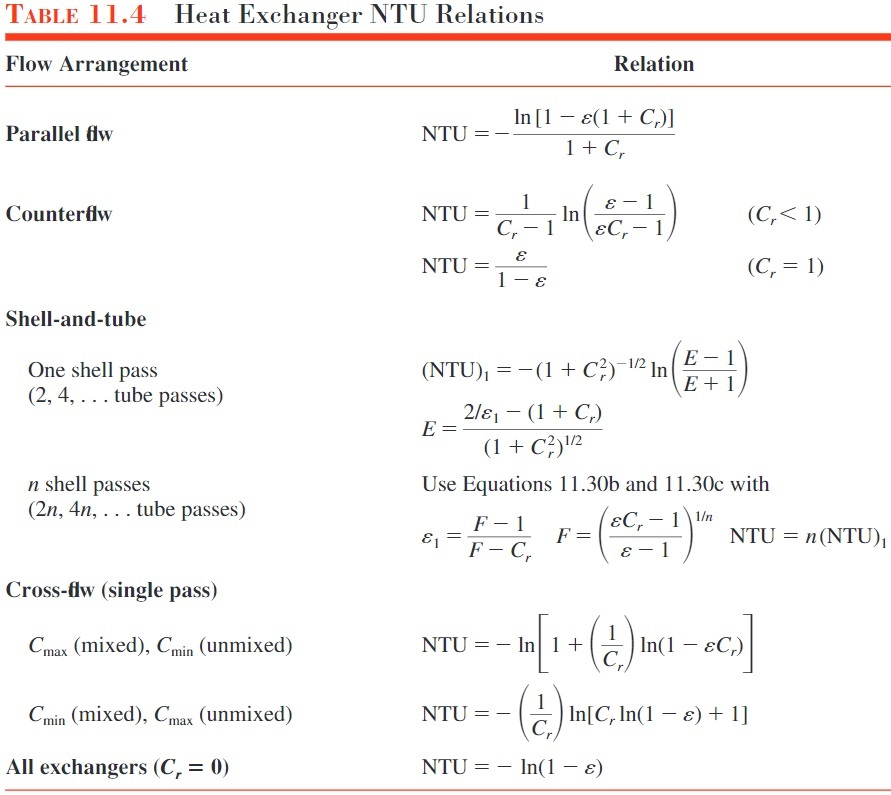
\includegraphics[scale=0.40]{Table11_4.jpg}
    \label{fig:Table114}
\end{figure}
\vspace{-20pt}
\begin{figure}[h!]
    \centering
    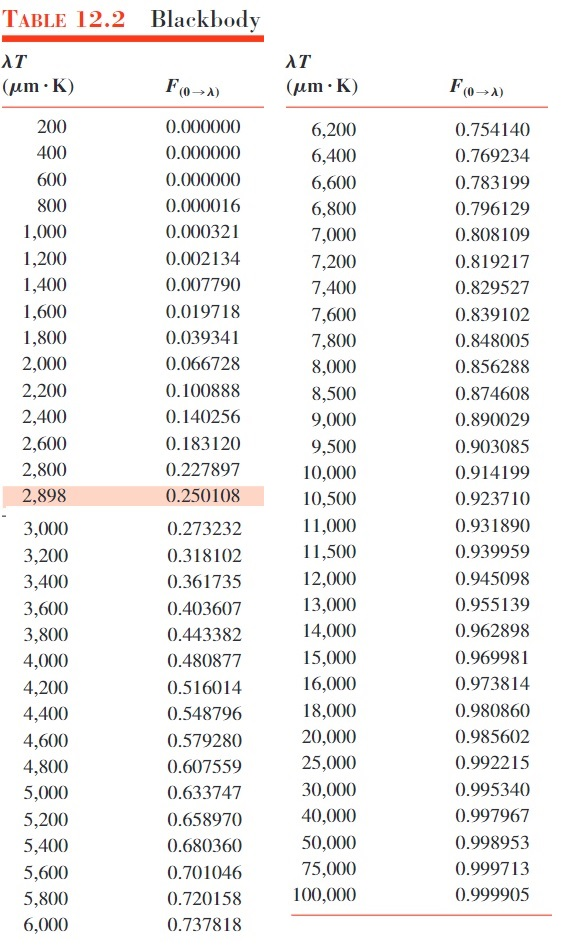
\includegraphics[scale=0.45]{Table12_2Compact.jpg}
    \label{fig:Table122}
\end{figure}

\end{document}